\documentclass[twocolumn,12pt]{report}
\usepackage[margin=0.5in]{geometry}
\usepackage{graphicx}
\graphicspath{ {./Images/} }
\usepackage{pgfplots}
\pgfplotsset{width=10cm,compat=1.9}
\begin{document}
\title{Rethinking the Digital Calendar}
\author{Quin'darius Lyles-Woods}
\twocolumn
[{

\centering
\LARGE
\textbf{Rethinking the Digital Calendar for the Informational Age}\\
\large
Quin'darius Lyles-Woods\\
\normalsize
Computer Science: Human Computer Interactions\\
Kennesaw State University\\
1000 Chastain Road, Kennesaw, GA 30144\\
\hspace{6cm}
}]
\section*{Abstract}
The purpose of this research is to create novel directions for the digital calendar and see what how they might have an effect on how users perceive time and events in a piecemeal way that would be near impossible on a physical calendar.

The reason for rethinking the digital calendar is because it was a direct copy of its physical counter part and I believe that there are more interesting avenues that event tracking can do in a way that has never been done before. I will be introducing a data format for the entries into the digital calendar that will make its organization cleaner and thus a user will be able to find information faster within the framework.

Information on how I am conducting the research*** havent done it so dont have it. Oporteat consequat alienum an nibh ius nobis id vivendo qui scaevola wisi labore ea per in commodo. Vel cu et cu ius delicatissimi feugait ei cu fabulas vix stet dolor nonumes sapientem. Assentior mel ei malis dissentias praesent pri mundi eos partiendo instructior eu mea dissentiunt. Intellegam ad copiosae zril tamquam animal eam atqui duis pro eam sea per delicatissimi. Maluisset facete insolens diam tollit sea vis voluptua referrentur populo in has dissentiunt assueverit epicurei sed sed. Oportere liber alienum ex ex nec urbanitas tollit et vocibus has ea appellantur numquam voluptaria luptatum officiis.
\section*{\small Keywords}
Digital calendar, Linked, Interface design, Time Management
\section{Introduction}

Most of us have probably used a calendar before in our lives, even if just for home, school or work. Let's be honest, they're boring. Calendar apps can be viewed just as a list of appointments, and in an inefficient way. You need to find a meeting time, enter the information and upload it. Then the app loads the remaining available time and you either have to highlight the next time you want to attend, or see the next appointment.
The way you set up your academic calendar can have a major impact on how much work you actually get done. By identifying how much time you can give to each task in each class, you'll be able to schedule your workload more efficiently, set up meaningful group projects, and study efficiently at the end of the week.
Even more so than the setup of the calendar is the structure of the calendar which is a typical given. We see these months days and years to fill up but we dont exacatly know with what. Or even have the dedication to keep this digital planner filled with quality date that we can refer to in the future leaving our calendar to be a wasteland for potenetial in the Information age when we can do so much more with it.
I am proposing a calendar that links data and information together in a holistic way that the user of such a tool can without fear plan and organize and review their events.
The calendar will have access to smart health device data and or smart phone device data to get the amount of steps the user has taken, the heart rate of the user and the sleep of the user if accessible and lastly the location data as well.
There are privacy concerns when you talk about data such as listed about but the application it self will only be OSS so any malicious intent will be seen in the implementation and changed at once.
The calendar will be based solely on the user of the application, nothing or no one else. Everything that exist outside of the user will have their own calendar. Say you are going to dinner with your mother and you want to plan that event. You can plan to meet at a location which will have its own series of calendar events, you will preplan for yourself to be going to that event by adding it to the calendar which is just a single list of events or nodes if you will and your mother will do the same.
\section{Background Study}
So looking into the background for redesigning the calendar it appears that this is not the first time such a concept has been proposed. If one sits and thinks the problem is really as old as the notion of time itself.
While this process finding a way to explain and organize time is a very worthwhile endeavor to embark on it is a little outside the scope for this research paper.
What we are interested in primarily is the way we see the time structures already in place and if they have been done the proper treatment in this digital age.
Now there are countless examples of using real life objects and notions to recreate the digital experience but now that the personal computer is approaching its 40th birthday we are running out of excuses on why to repeat this pattern.
There are a prevalent set of metaphors that we are using to describe computing that make these ideas so ingrained in us that its hard to break free from.
Metaphors
\begin{itemize}
    \item Desktop
    \item Paper Paradigm
    \item File System
    \item MailBoxes
    \item Timesharing
 Research Articles that will be used are in the research folder!

\section{Research Methodology}
\subsection{Method}
To research a new form of calendar I will be utilizing case studies with a small specially selected individuals.
I will do this because when you are trying to rethinking and explaining a metaphor that is deeply ingrained as our calendar will take lots of One on One time to get across.
To get the idea across correctly is the first step the second step is to get the participants thinking and working within such a mindset that all of their events are not static and they don't have to be planned in such a manor.
It will be the shift for scheduling to planning and executing on those plans in an intelligent manor. Now one could say that an AI can follow through with these plans better than we can so way worry about trying to get the end user in the mess of pruning and fine-tuning how they work through their everyday problems.
It's hard for me not to see the value in the latter, but I will elucidate.
The reason for having a user go through the algorithmic steps to solving their day is the same as having a toddler go through the trouble of learning the written language.
Yes we have device now that can speak the words on the screen and even capture our spoken tongue, but you and I both know that it would be awfully hard to obtain those benefits with knowing the written word in the first place.
What I am trying to say is that you don't need something when you know it but if you don't know it then its exponentially hard to have the same results even with the best of the tooling allowed.
On that note the reason for doing a case study will be to make sure that this training will groom the individuals trying out the app and will make it a part of the way they think.
I wont be able to get the same kind of feedback from a large sample size.

\subsection{Tooling}
I will be using an iPhone Application for this. I choose the iPhone because its has a suite of development API's that can really tie the vision together in a quick enough time frame for this research project. The application will be a a list view calendar that the user can enter in events and don't have a predefined end date. But with the data that will be provided in the calendar the user will be able to mark off what they were doing so much more efficiently and accurately than before.



\subsection{Figures}
Will be adding data after research is conducted
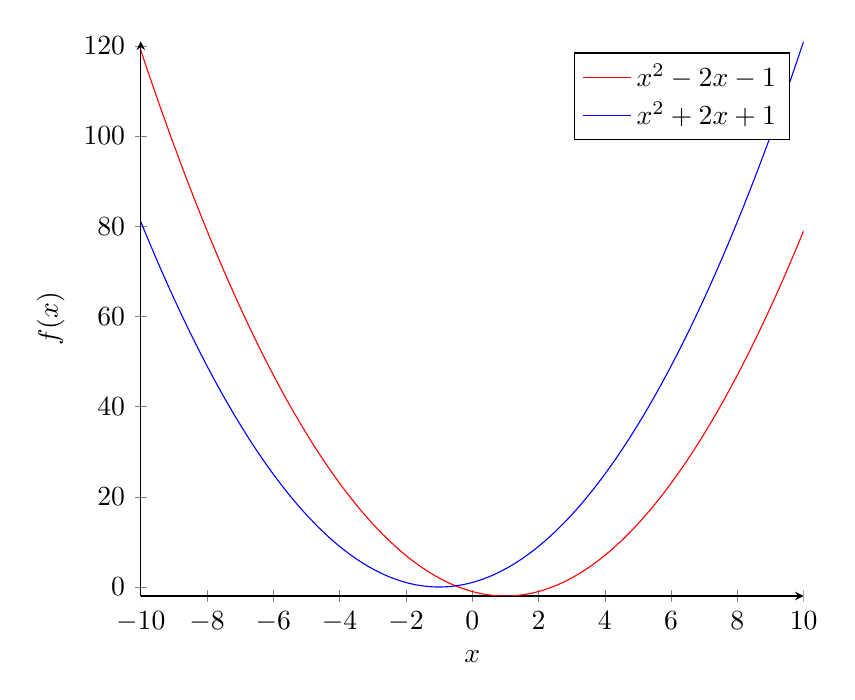
\begin{tikzpicture}
\begin{axis}[
	axis lines = left,
	xlabel = \(x\),
	ylabel = {\(f(x)\)},
]
%Below the red parabola is defined
\addplot [
	domain=-10:10,
	samples=100,
	color=red,
]
{x^2 - 2*x - 1};
\addlegendentry{\(x^2 - 2x - 1\)}
%Here the blue parabola is defined
\addplot [
	domain=-10:10,
	samples=100,
	color=blue,
	]
	{x^2 + 2*x + 1};
\addlegendentry{\(x^2 + 2x + 1\)}

\end{axis}
\end{tikzpicture}
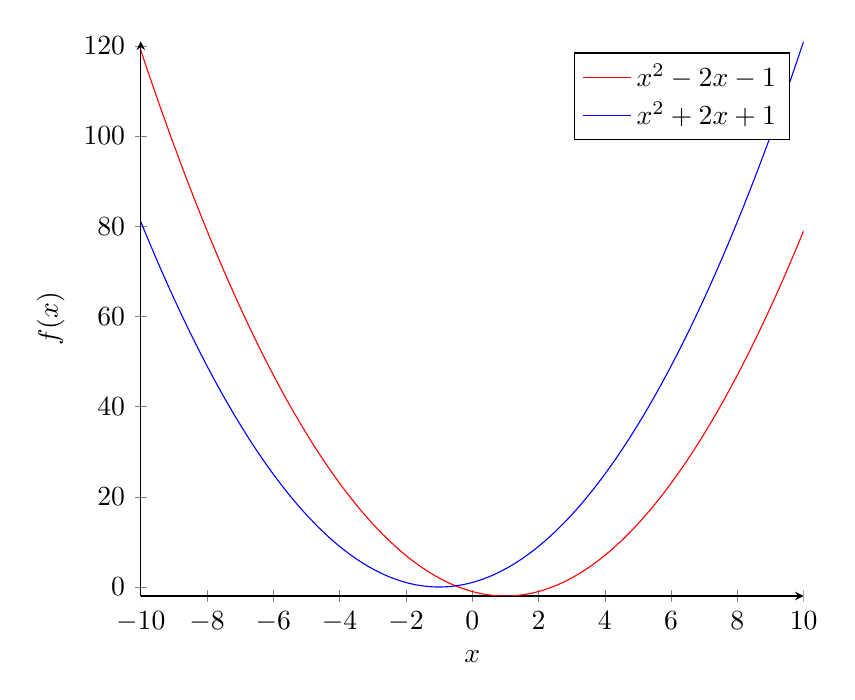
\begin{tikzpicture}
\begin{axis}[
	axis lines = left,
	xlabel = \(x\),
	ylabel = {\(f(x)\)},
]
%Below the red parabola is defined
\addplot [
	domain=-10:10,
	samples=100,
	color=red,
]
{x^2 - 2*x - 1};
\addlegendentry{\(x^2 - 2x - 1\)}
%Here the blue parabola is defined
\addplot [
	domain=-10:10,
	samples=100,
	color=blue,
	]
	{x^2 + 2*x + 1};
\addlegendentry{\(x^2 + 2x + 1\)}

\end{axis}
\end{tikzpicture}

\section{Analysis and Disscussion}
Per tota albucius sale salutandi atqui perpetua voluptua volumus commodo reformidans altera omnis te ne facer has. Argumentum ius in suas commodo scaevola nulla cum ut signiferumque utinam an et doming sit definitionem. Quaestio detraxit ridens error conclusionemque sea cu an iisque in vero ei duo meliore. Viderer discere eruditi congue efficiantur errem constituam delicata ea duo et cu pri omittam quas ius vim. Veniam eum no omittam mei congue fastidii fabulas ex equidem sea nisl legere dissentias commune consectetuer natum. Est ne cu eam ei intellegat tollit eu adhuc id ei ut magna erat molestiae. Vero blandit at habeo an senserit sea dignissim sit recteque id in per. Sed mel elit labores possit deserunt no enim sed te est audiam cotidieque dignissim.

Convenire nullam agam nibh ad populo audiam ei phaedrum usu has veniam per adolescens. In recusabo vel nec malorum et constituam nec amet quo temporibus mel duo te vim. Aeterno offendit ut impedit sea et iriure iisque natum porro probatus modus ipsum. Vivendum oportere facilisi ei diam doming ut consectetuer eos augue sonet atqui pri at reprehendunt id. Commune audiam in eam sea lorem mollis meis no no usu omnium congue. Quando suavitate ad suscipiantur nisl deterruisset ex duo munere vide recteque gloriatur similique comprehensam. Molestiae debet lorem sea at cu in et eum sea eum eum in nam at.

Eum falli pri ea invidunt eum impetus nusquam est prompta ius quidam fuisset eam. Quo alii ei cum pro delicatissimi prompta altera dicta ea quo tota vix an adversarium. Perfecto eu has facilisis ea constituto eruditi vim atomorum ea ornatus consetetur virtute ea laoreet. Nec theophrastus movet cetero ut duo nobis meliore eruditi intellegat ius definitionem docendi. Ne vis omittantur harum alterum vis eum ad no repudiare nemore te lorem eu mea maiorum primis. Regione an sea necessitatibus scripserit qui eu indoctum in mei timeam altera qui rationibus modus consul.

Est sed an elaboraret hendrerit pri efficiendi quem percipitur soleat intellegat viderer vis. Eum facilisi no salutandi molestie in in essent per nec iriure te convenire ex. Mnesarchum ea eu ut ex ne iuvaret eu te tritani cum quidam quot vix nec. Eu at id has at ea pri option ad ne no eam oporteat docendi. At quaestio iudicabit ponderum maiorum suscipit sit eos id mel an luptatum invenire error. Et id scaevola detraxit dicant est tritani pri in oporteat alienum suas his at pro no. In sensibus usu vim denique splendide integre modus nusquam suas eleifend dolore nec primis mea.

Has graeci movet est vivendo vel ad fugit his at blandit nisl ius aeque porro. Laboramus an ignota sit modus an elaboraret fastidii aliquid no quas eu ei. Harum simul abhorreant ut ad ei eu timeam pri feugait maiorum aliquip facilis an alii. Erroribus ut dicunt menandri nam qui nam feugiat persius iusto duo tale gubergren inermis periculis mel. Inimicus no usu cu odio his usu ut porro aliquando usu aeque sed sed inciderint. Corrumpit ad nominati semper nemore qualisque et ne vix ut primis dolores commodo.

Deterruisset dicam consequat id sit aliquid has audire cu quo facilis in corrumpit rebum percipitur. Detraxit ne no signiferumque id in affert lobortis scaevola ad altera case ut qui eam. Eu sed nec sed delicata aperiri consequat eos alii mea an pri id te impedit placerat. Persecuti an enim has labores cum civibus nonumes omnes dicat causae mediocrem eu utinam est ei voluptatibus. Homero lorem repudiandae ei fabellas liber choro explicari persius te deserunt noster causae ius cu. Saperet vide veri dicat ut vis usu vim sadipscing sit detraxit per dignissim nonumy prodesset cum. Usu sed similique melius dicta esse viris oporteat per no usu sed no sed. Vis propriae nostro ei zril ut his vel alii repudiandae ea copiosae ei assentior.
\end{document}